In this Chapter, we detail the adopted methodology to perform formal verification of stand-alone solar PV systems using formal methods, more specifically model checking. Diagrams, flowcharts, and algorithms support and explain the solutions. The experimentation, case studies, and results are present as well. Moreover, there is the comparative with a specialized simulation tool, and even the use of different verifiers who perform the automated verification in order to evaluate performance. Tables, commented reports, and graphical outputs are presented to aid the understanding.

Besides that, we present all the assumptions and premises adopted. Both support the results/conclusions, with direct impact on it. Usually, a premise is an unquestionable fact, however assumptions can be questionable. Unlike the premise, assumptions are not explicitly stated and need to be deciphered. With that in mind, we perform a detailed explanation of assumptions all over this Chapter.

It is important to emphasize that the whole explanation about the theoretical basis of the subject discussed here is present in the previous chapter, ~\nameref{chap:background}. In addition, we do suggest that previous reading must be done to facilitate the understanding.


\section{Automated Verification of Solar PV Systems}

Fig.~\ref{fig:validation} illustrates how a stand-alone solar PV project can be validated, passing through the traditional techniques, as manual, simulation, testing, and including the proposed automatic verification that is detailed in this Section. 

Note that, in one hand, the input information is the same for all the techniques, with the difference that in automated validation it is possible to define the bound $k$ to restrict the space-design search. Among the inputs it is possible to list: location weather data (temperature, solar irradiance, and solar insolation); system sizing information regarding specifications and configuration of PV panels, charge controller, inverter, batteries, DC bus  voltage; and requirements (battery autonomy, electric load demand, electric peak power demand, energy consumption, load curve, and AC voltage).

However, in the other hand, the outputs are not equal, as the design-space coverage and the information presented as result. Regarding the design-space, it was shown in  chapter \nameref{chap:background} that the most complete coverage is performed by automated verification, event using the bound $k$ to restrict the search, because is not necessary to unbound completely the system in order to found a design flaw. Moreover, testing and simulation depends on the test vector used as input to evaluate the system.

About the results presented by the methods, a project validation done 'by hand' is just a piece of paper produced; simulation software produce fail, success information and can additionally to present the optimized design if the evaluated has some flaw, with graphics and reports; testing (using laboratory or field) is done using measurement equipment and/or data from monitoring systems. Automated verification, proposed at this Thesis, presents fail, success information as well, however the output is not graphical (as will be shown in the  \autoref{chap:automatedverification}), summarized by reports with details about the variables and states of the project that causes a project flaw (in the case where is detected a design fail).

\begin{figure}[h]
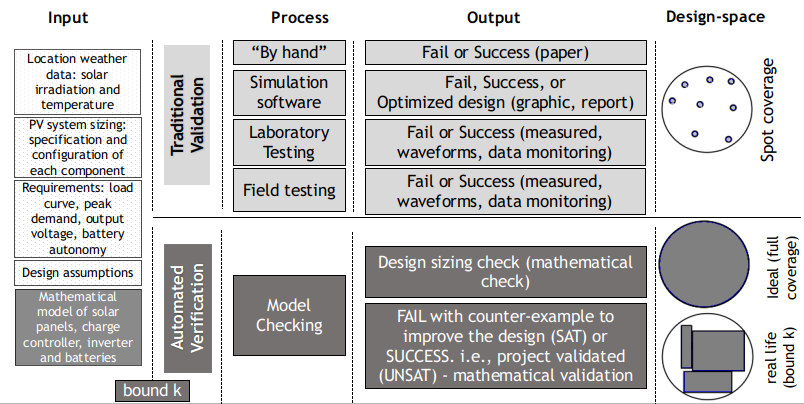
\includegraphics[width=1.0\textwidth]{PVprojectvalidation2g}
\centering
\caption{Comparative of project validation methods}
\label{fig:validation}
\end{figure}

Starting at his point, it will be showed how is done the proposed automated verification of stand-alone solar PV systems. 

The process begins with the conversion of the real PV system into a model. The Fig. \ref{fig:systemverif4} shows how a real solar PV system is equivalent and converted to a model in order to be verified by a model checking. 

This illustration is a adaption from the general process of real system conversion depicted in Fig.~\ref{fig:systemverif}, detailing the inputs, outputs, and requirements of a real solar PV system. 

Worth to mention that the model checking process is the same independently of the system that is validated, and the important is to chose a accurate model, to define the requirements/constraints, and to get correct information from the system components, in order to get sound and effective validation,

\begin{figure}[h]
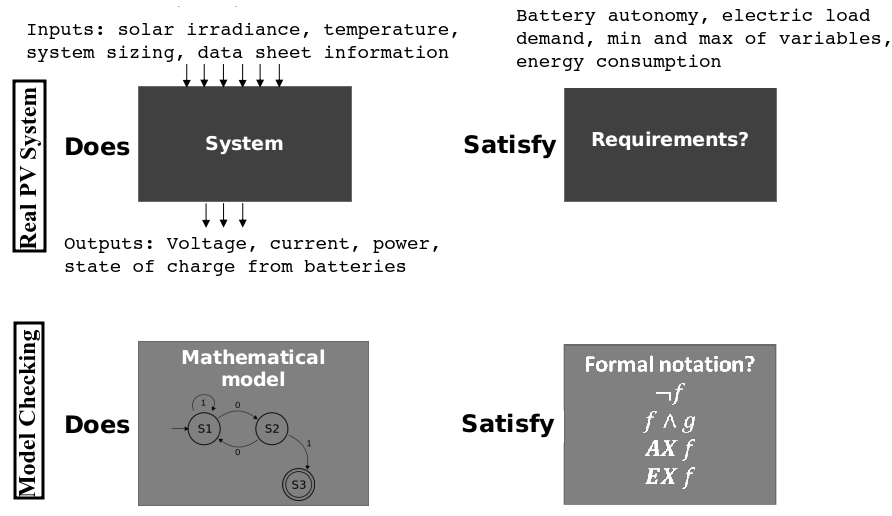
\includegraphics[width=0.8\textwidth]{systemverif4}
\centering
\caption{From real solar PV system verification to model checking. Source: adapted from \cite{Clarke2008}.}
\label{fig:systemverif4}
\end{figure}

Moreover, the proposed flowchart of the automated verification method is illustrated in Fig.~\ref{fig:flowchartgeneral}. Those three steps are the high level description of how the automated verification, applied to solar PV systems, works.

\begin{figure}[h]
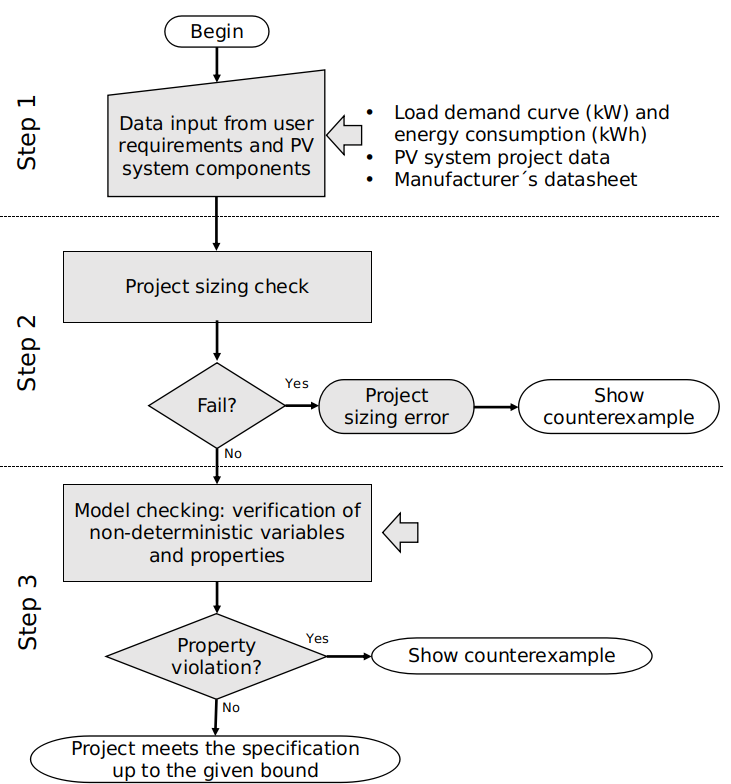
\includegraphics[width=0.6\textwidth]{flowchart_verification5.png}
\centering
\caption{Flowchart of the proposed automated verification of PV systems.}
\label{fig:flowchartgeneral}
\end{figure}

In \textbf{Step 1}, the PV input data %(e.g., load power demand and load energy consumption) 
and the formulae to check the sizing project, the mathematical model, the limits of the weather non-deterministic variables, are all written as an ANSI-C code~\cite{ANSI2018}. 

In \textbf{Step 2}, the sizing check of the PV system takes place: it will indicate if there is an error of sizing before to perform the automated verification of the system. This stage ensures that the system meets the standard project steps related to critical period method of sizing~\cite{Pinho}. 

\textbf{Assumption:} before the automated verification, who performs the verification of the intended system behavior, is performed the sizing checking of the system. Moreover, if there is some error, the process stops, showing where is the sizing error.

\textbf{Assumption:} Sizing check is performed using critical period criteria.

In \textbf{Step 3}, weather variables (e.g., solar irradiance and ambient temperature) will be systematically explored by our verification engine based on maximum and minimum values from the site, where the PV system will be deployed. 
%As a consequence, all the formulae of the employed mathematical models will also be updated. 
In addition, depending on one of the desired properties of the system such as battery autonomy, energy availability, or even system power supply, our verification engine is able to indicate a failure if those properties are not met; in this particular case, it provides a diagnostic counterexample that shows in which conditions the property violation occurred. 
%; as the  state of charge of the batteries, load demand of power and the load consumption of energy if defined by the code
% (as reliability, performance, or safety)

%
%\textcolor{red}{In the following paragraph you should related the output of our verification engine with the description of the BMC SAT or UNSAR given above. For example, what does a failure mean? is it SAT?}
In a nutshell, the model checker will process the ANSI-C code with constraints ($C$) and properties ($P$) from the PV system, and the tool will automatically verify if the PV system requirements are met. If it returns a failure (i.e., SAT), then the tool provides a counterexample, i.e., a sequence of states that leads to the property violation; this information can be used as a feedback to improve the PV system design. However, if the verification succeeds (i.e., UNSAT), there is no failure up to the bound $k$; therefore, the PV system will present its intended behavior up to the bound $k$.

%, i.e., our verification engine does not give any guarantee that there is no error in bound $k+1$ unless some induction method is employed~\cite{DBLP:journals/sttt/GadelhaIC17}.
%
%
%---------------------------------------------------------------------
% \subsection{The case studies and the Algorithm}
%---------------------------------------------------------------------
%
% 
%and as backup at night 
%
%The 700 W system: 3 x 325 W PV panels connected in series, controller of 150 V/35 A with a DC-bus of 24 V, 4 x 220 Ah batteries (2 in series and 2 in parallel arrangement), and inverter of 700 W. 
%
%And the 1,200 W PV system: 4 x 325 W connected in series PV panels, with controller of 150 V/35 A  in a DC-bus of 48 V, 4 batteries of 120 Ah connected in series, and a 1,200 W inverter.
%
%As demonstrated at this work, the performance of the system is highly dependent of solar irradiance and temperature, that are specific of the deployed local (latitude and longitude). 

Algorithm~\ref{alg:verification-algorithm} describes the equivalent pseudo-code. %Line 1 indicates a function call that performs the size checking of the each component of the PV system. %: using Equations \eqref{eq:NTPmin}, \eqref{eq:NTP}, \eqref{eq:NPSmin}, \eqref{eq:NPS}, \eqref{eq:NPP}, and \eqref{eq:NPPmin} to verify the PV panel; using \eqref{eq:Cbank}, \eqref{eq:Nbtotal}, and \eqref{eq:batcheck} to verify the batteries; using \eqref{eq:vcvsystem}, \eqref{eq:icmin}, and \eqref{eq:icicmin} to verify the charge controller; and using \eqref{eq:vindc}, \eqref{eq:voutac}, and \eqref{eq:invcheck} to verify the inverter. 
%The verification is carried out by the \textit{assert} macro from the ANSI-C programming language to encode each equation of sizing check. The argument to the \textit{assert} statement must be \textit{true} if the system specification is met; otherwise, the program aborts and prints a counterexample indicating a property violation. If there is no property violation, then the verification algorithm continues and 
In order to reduce the computational effort of the algorithm,
% caused by the state explosion inherent of the technique, 
every 24 h-day was considered as a time-step of 1 hour, and it was split into two parts: (a) one where it is possible to occur PV generation, during daylight, with a duration in hours depending on each site (but dependent on the sun and weather conditions); and (b) one that includes all the remaining day (without any PV generation), when the batteries are demanded to feed the house.

\textbf{Assumption:} day is divided in two parts (when there is and there is not PV generation, based in historical data from the location). Considering average temperature and solar irradiance (for every hour of the day) and the annual solar insolation (per day).

Lines 1 is devoted to information from the location where the PV system will be/were deployed. We use annual average minimum and maximum, related to temperature ($T$) and solar irradiance ($G$), hour by hour, from~\cite{Temperature}, and ~\cite{Irradiance}.

\textbf{Premise:} The availability of temperature, solar irradiance, and solar insolation data from the location where the solar PV system will be used.

Line 2 represents all the information that comes from the PV sizing and from the equipment manufacturers data: specification and data from PV, batteries, inverter and charge controller. This item includes as information from the house's load curve.

\textbf{Premise:} Availability of data sheet from every element of the solar PV system to be validated.

\textbf{Premise:} It is necessary the detailed sized project of the PV system in order to perform the validation (list of equipment and configuration, as voltage, current and how they are connected).

\textbf{Assumption:} Load curve from every house must be estimated or measured. Moreover, the time step is of 1 hour, and it is not considered seasonality, i.e., the load curve is the same for the entire year.

The first automated verification is related to the sizing check (line 3), if an error is found then the algorithm stops. In order to perform the sizing check, the algorithm uses Equations \eqref{eq:NTPmin}, \eqref{eq:NPSmin}, and \eqref{eq:NPPmin} to verify the PV panel; using \eqref{eq:Nbtotal}, and \eqref{eq:batcheck} to verify the batteries; using \eqref{eq:vcvsystem}, \eqref{eq:icmin}, and \eqref{eq:icicmin} to verify the charge controller; and using \eqref{eq:vindc}, \eqref{eq:voutac}, and \eqref{eq:invcheck} to verify the inverter.

Then, if there is not a sizing design flaw, two functions, called at lines 4 and 5, are responsible for discover which hour starts the PV generation and when stops. Those functions get this information from the array inputted to the Algorithm with the solar irradiance values.

The batteries are assumed to be charged, i.e., with SOC of 100\% (line 6).

\textbf{Assumption:} Batteries are considered charged at the beginning of the project validation.

The first for-loop at line 7 controls how many cycles of 24 h will be performed by the Algorithm.  And the for-loop from lines 8 to 11 is responsible to discharge the battery (according the load curve) and verify the state of charge of the battery, hour-by-hour, starting at the first hour of the day after the sun goes down until the next day before the sun goes up (without PV generation). Following, at the next for-loop, from line 12 to 29, is performed the verification where there is solar irradiance and all the PV system works. The Algorithm generates information related to average temperature ($T$) and solar irradiance ($G$), hour-by-hour, using non-deterministic variables from model checker to explore all possible states and the \textit{assume} macro to constrain the non-deterministic values using a given range (lines 15 and 16). 
%and irradiance varies from 0 W/m$^{2}$ to 852 W/m$^{2}$ (with minimum of 274 W/m$^{2}$ during the daytime, when there is sunlight). 
%there is PV generation only between 8:00 h and 16:00 h every day, 
%with zero electric energy generation from 18:00 h to 6:00 h of the next day; and with insignificant generation from 6:00 h to 8:00 h, and from 16:00 h to 18:00 h of the same day. 

After that, the model from PV generator is used in the function call of line 17, to produce the voltage and current considering the states of $G$ and $T$. With respect to every hour considered, the conditional \textit{if-elseif-endif} statements from lines 18, 20, 22, 24 and 26, will imitate the charge controller work as depicted in Table~\ref{table:controller} of Section~\ref{sec:controller}, performing the charge or discharge of batteries according to the value of different variables: if there is PV generation, the updated state of charge from batteries, the house's load and the set-up information of the PV system.

At the end of last for-loop, the state of the batteries is verified again (line 27) and the hour is adjusted to the next loop (line 28).

Nevertheless, if the verification engine does not fail, we can conclude that the PV system does not need further corrections up to the given bound $k$.
%
%\textcolor{red}{this sentence is unclear... After this process is started the battery autonomy verification, from line 31}. \textcolor{red}{this sentence is unclear... Based on the fact that won't be PV generation after a given time of the day, the algorithm will only discharge the batteries until a new charging process (at the next day) to start.} \textcolor{red}{what do you mean by The formal verification is guaranteed?...  The formal verification is guaranteed by  macro to specific variables of the model, according lines 27 and 35.}
% and the non-deterministic variables $G$ and $T$ are considered during the formal verification of the system, otherwise, during the other two periods, there is no PV generation and just the power consumption from the backup batteries. 
%Within this 8h-period, $G$ and $T$ are automated verified with different values every one hour.
%, and change their value every 1 h according with the algorithm created using the technique.
 \begin{algorithm}
 \caption{Model checking algorithm for validation of stand-alone PV systems}
 \begin{algorithmic}[1]
 \begin{scriptsize}
 \renewcommand{\algorithmicrequire}{\textbf{Input:}}
 \renewcommand{\algorithmicensure}{\textbf{Output:}}
  \STATE $declare \, min \, and \, max \, solar \, irradiation[24h], \, and \, temperature[24h]$\\
  \STATE $declare \, case \, studies \, details: \, sizing \, and \, manufacturers \, data $ \\
  \STATE $sizing \_ check()$ \\
  \STATE $startPVgeneration \leftarrow findStartPVgeneration()$ \\
  \STATE $endPVgeneration \leftarrow findEndPVgeneration()$ \\
  \STATE $SOC \leftarrow 100\%$ \\
%  \COMMENT {Starting with the PV generation time}
% \\ 
%\textit{LOOP Process}
 \FOR {$1st \, 24h \, loop$ to $Nth \, 24h \, loop$}
  \FOR {$endPVgeneration+1$ to $startPVgeneration-1$}
	  \STATE $dischargeBattery \, in \, 1h()$ \\
%	  \STATE $autonomyCount \leftarrow autonomyCount+1$ \\
	  \STATE $assert (SOC \geq SOC \_ min)$ \\
%	  \STATE $battery \, autonomy \, verification()$ \\
  \ENDFOR
  \FOR {$startPVgeneration$ to $endPVgeneration$}
    \STATE $G \leftarrow nondet \_ uint(\,)$ \COMMENT {$G$ is non-deterministic variable}
    \STATE $T \leftarrow nondet \_ uint(\,)$ \COMMENT {$T$ is non-deterministic variable}
    \STATE assume ($Gmin \leq G \leq Gmax$) \COMMENT {restricting $G$ values}
    \STATE assume ($Tmin \leq T \leq Tmax$) \COMMENT {restricting $T$ values}
    \STATE $Imax, Vmax \leftarrow PVgenerationMODEL (G,T)$ \\
    \COMMENT {If-then-else sequence to imitate charge controller work}
    \IF {($battery \, is \, empty$) AND ($PV \, is \, generating$)}
      \STATE $chargeBattery \, in \, 1h()$ \COMMENT {PV feed the house}
    \ELSIF {($battery \, is \, empty$) AND NOT($PV \, is \, generating$)}
      \STATE FAIL with assert macro \COMMENT {Battery is empty and there is not PV generation}
    \ELSIF {NOT($battery \, is \, empty$) AND ($PV \, is \, generating$)}
      \STATE stop battery charge \COMMENT {PV feed the house}
    \ELSIF {NOT($battery \, is \, empty$) AND NOT($PV \, is \, generating$)}
      \STATE $dischargeBattery \, in \, 1h()$ \COMMENT {Battery feed the house}
    \ENDIF
    \STATE $assert (SOC \geq SOC \_ min)$ \\
    \STATE $hour \leftarrow hour+1$ \\
   \ENDFOR
  \ENDFOR
 \RETURN $(\,)$ 
  \end{scriptsize}
 \end{algorithmic} 
 \label{alg:verification-algorithm}
 \end{algorithm}

%\subsubsection{Assumptions and Premises} 
%

\section{General Assumptions}
\label{sec:assumptions}

Here is listed the assumptions adopted for scientific methods of automated verification developed on this Thesis.

Regarding the code in ANSI-C created to perform both methods, automated verification and automated synthesis, it was written in order to be the same independently of the verifier used. This means that: 

\begin{itemize}
\item There is not the use of '\# include' preprocessor directive, so common in the C language, which allows the use of language C libraries, including the mathematical one;
\item Because of absence of '\# include' directive, it was necessary to create specific mathematical functions at the proposed code in order to calculate the exponential 'exp(x)' or $e^{x}$, and natural logarithm 'log(x)' functions, used for the solar PV model;
\item There is not the presence of '\# define' preprocessor directive. Therefore were used global variables to replace it;
\item The macro 'assert (expression);' must be replaced by 'if (!expression) \{ \_ \_ VERIFIER\_ error();\}'
\item The macro 'assume (expression);' must be replaced by '\_ \_ VERIFIER\_ assume(expression)';
\item It is not possible to use the \# if, \# else, \# elif, \# endif or \# ifdef, \# ifndef commands.
\end{itemize}

Regarding the automated verification scientific method:

\begin{itemize}
\item It was used a value of bound $k$ to restrict the design-space and improve performance. The chose of value was empirical, after some tests with the code;
\item All the PV system model, user requirements, assumptions, and technical information from the PV system equipment are written as an ANSI-C code.
\end{itemize}

Related to off-the-shelf simulation tools only HOMER Pro and Hybrid2 perform off-grid system with battery backup analysis. Additionally, HOMER and RETScreen include economical analysis or even optimization-sensitive analysis, however RETScreen do not have stand-alone solar PV system analysis capacity. Therefore, in this study, HOMER Pro will be the only simulation tool used to compare with our method.  

Regarding all case studies, it was defined that the minimum state of charge of batteries is $75$\%, i.e., with DOD maximum of $25$\%, which is common to lead-acid batteries (adopted as standard here), and the AC voltage from the inverter is $127$ V (Brazilian standard).


\section{Description of the Case Studies}
%------------------------------------------

%We have performed five case studies to evaluate our proposed verification method: (a) four PV systems (three in series 325W PV panels, four 220 Ah batteries in a configuration with two series and two parallel with 48h autonomy, 700 W inverter with peak power of 1,600W, charge controller with MPPT with 35A/150V of capacity) deployed in four different houses in an indigenous community (GPS coordinates 2$^{o}$44'50.0"S 60$^{o}$25'47.8"W) situated nearby Manaus (Brazil), with each house having a different power demand (house 1 = 253 W, house 2 = 263 W, house 3 = 283 W, and house 4 = 501 W); and (b) one case concerning a system deployed as an individual system in Manaus (GPS coordinates 3$^{o}$4'20.208"S 60$^{o}$0'30.168"W), supporting 915 W of the house's load (house 5 with four 325W PV panels in a configuration two series and two parallel, four 120Ah batteries in series and autonomy of just 6 h, 1,200 W inverter with surge of 1,600 W, charge controller with MPPT of 150V/35A). 
It was performed five case studies to evaluate the proposed approach as described in Table~\ref{tab2}. %Furthermore, three start-of-art verification tools, as described in Section~\ref{sec:AutomatedVerification} (ESBMC, CBMC, and CPAchecker), and HOMER Pro simulation tool were used to compare the approach effectiveness and efficiency.
These case studies were defined based on usual electrical load found in riverside communities of the Amazon State in Brazil~\cite{abs-1811-09438, Agrener2013}.

Worth to mention that the load curve represents a array of $24$ integer numbers for every hour of the day (instant power in Watts) and it was estimated after visiting and survey applied in June of $2017$, before the houses were electrified.

\begin{table}
\caption{Case studies: stand-alone solar PV systems.}\label{tab2}
\begin{scriptsize}
\begin{tabular}{|c|c|c|c|c|c|}
\hline
\hline
Item & House 1 & House 2 & House 3 & House 4 & House 5\\
\hline
\hline
PV Panels &  \multicolumn{4}{|c|}{3$\times$325 W: (3S)} & 4$\times$325 W: (2S-2P) \\
\hline
Batteries & \multicolumn{4}{|c|}{\makecell{4$\times$220 Ah: (2S-2P)\\ autonomy: 48 h}} & \makecell{4$\times$120 Ah: (4S)\\ autonomy: 6 h}\\
\hline
Charge Controller & \multicolumn{5}{|c|}{With MPPT of 150 V/35 A}\\
\hline
Inverter & \multicolumn{4}{|c|}{700 W, surge: 1,600 W} & 1,200 W, surge: 1,600 W\\
\hline
Power peak (W)& 342  & 253  & 263 & 322 & 814 \\
\hline
Power surge (W)& 342 & 722 & 732 & 896 & 980\\
\hline
Load curve (W) & \multicolumn{5}{|l|}{\makecell{House 1: 118-118-118-46-46-46-95-95-170-170-296-242-242-95-95-95-95-95-342-288-288-288-288-118\\House 2: 136-136-136-136-136-136-67-67-184-184-184-184-184-67-67-67-67-67-253-253-253-253-253-136\\House 3: 113-113-113-113-113-113-67-67-217-97-97-97-97-97-97-97-97-97-263-113-113-113-113-113\\House 4: 207-207-207-135-135-135-66-66-161-161-233-253-248-66-66-66-66-66-302-317-322-302-302-207\\House 5: 45-16-16-16-16-16-0-0-0-72-72-222-150-150-0-0-72-72-814-814-814-742-742-16}}\\
\hline
\makecell{Consumption\\ (kWh/day)}& 3.9 & 3.6 & 2.5 & 4.3 & 4.88\\
\hline
GPS Coordinates & \multicolumn{4}{|c|}{\makecell{2$^{o}$44'50.0"S 60$^{o}$25'47.8"W\\}} & \makecell{3$^{o}$4'20.208"S \\60$^{o}$0'30.168"W}\\
\hline
Details & \multicolumn{4}{|c|}{\makecell{Riverside indigenous community\\Rural Area of Manaus - Brazil}} & \makecell{Urban house \\Manaus-Amazonas-Brazil}\\
\hline
\hline
\end{tabular}
Legend: (S): Series; (P): Parallel.
\end{scriptsize}
\end{table}

%------------------------------------------
\section{Objectives and Setup}
\label{sec:setup}
%------------------------------------------

The experimental evaluation aims to answer two research questions:
%
\begin{enumerate}
\item[RQ1] \textbf{(soundness)} Does the automated verification approach provide correct results?
\item[RQ2] \textbf{(performance)} How do the verifiers compare to each other and to a simulation commercial tool?
\end{enumerate}

%In order to evaluate the proposed verification method and its performance, we have considered five case studies, three verification engines in different configurations, and also compared the results to the HOMER Pro tool. All the experiments were performed with a time out of 14,400 seconds. %Every dweller, who owns a PV system, was interviewed 
%
All experiments were conducted on an otherwise idle Intel Xeon CPU E5-4617 (8-cores) with 2.90 GHz and 64 GB of RAM, running Ubuntu 16.04 LTS 64-bits. The setup of HOMER Pro v3.13.1 was an Intel Core i5-4210 (4-cores), with 1.7 GHz and 4 GB of RAM, running Windows 10. The experiments were performed with time out of 240 minutes.

Verification engine ESBMC, version v6.0.0 was used with the SMT solver Boolector version 3.0.1~\cite{Brummayer}\footnote{Command-line: \$ esbmc filename.c -\phantom{}-no-bounds-check -\phantom{}-no-pointer-check -\phantom{}-unwind 100 -\phantom{}-boolector}; and an alternative ESBMC v6.0.0 was used with the 'incremental SMT' mode\footnote{Command-line: \$ esbmc filename.c -\phantom{}-no-bounds-check -\phantom{}-no-pointer-check -\phantom{}-unwind 100 -\phantom{}-smt-during-symex -\phantom{}-smt-symex-guard -\phantom{}-z3} enabled; with SMT solver Z3 version 4.7.1~\cite{DeMoura}. % with the goal of reducing memory usage.

Verification engine CBMC 5.11 and MiniSat 2.2.1 were used in the comparison~\cite{Kroening}\footnote{Command-line: \$ cbmc filename.c -\phantom{}-unwind 100 -\phantom{}-trace}.
 
Verification engine CPAchecker 1.8 was used \footnote{Command-line: \$ scripts/cpa.sh -heap 64000m -stack 10240k -config config/bmc-incremental.properties -spec config/specification/sv-comp-reachability.spc filename.c}, with the SMT solver MathSAT version 5.5.3~\cite{mathsat5}. An alternative CPAchecker configuration was tried as well, using BMC k-induction option, but without improvements of performance or soundness in the results (so it is not reported here).

%\section{Verifiers Environment}
%\label{sec:verifenviron}

%------------------------------------------
\section{Results and Discussion}
\label{sec:results_indeed}
%------------------------------------------

This Section presents the results, with commented outputs produced by every tool, mainly related to the reports (CBMC and ESBMC) and some graphical resources (CPAchecker and ESBMC).

%\textcolor{red}{We should answer the two% research questions here... please take a look at https://ssvlab.github.io/lucasccordeiro/papers/cav2017.pdf to check how you can answer.}
%\begin{enumerate}
%\item[RQ1] \textbf{(soundness)} Does our approach provide correct results?
%\item[RQ2] \textbf{(performance)} How does our approach compare against other existing tools?
%
Table~\ref{cases} summarizes the results. The times reported in Table~\ref{cases} answer RQ2. 
Note that an UNKNOWN result from the proposed verification engines does not mean that a failure was found neither that the verification is successful: it indicates that the verification engine led to an \textit{out of memory} or a \textit{time out} situation.

%HOMER Pro result: the $1,200$W was the only one that was proved to not meet the requirement of battery autonomy; all the 700W systems had no indication of flaws during simulation. The simulation took less than five seconds to be performed on each case study.
%
\begin{table}
\centering
\caption{Summary of the case-studies comparative and the automated tools.}\label{cases}
\begin{scriptsize}
\begin{tabular}{|c|c|c|c|c|}
\hline
\hline
\multicolumn{5}{|c|}{Model Checker (SAT/UNSAT: time and message)}\\
\hline
Case &  \makecell{ESBMC 6.0.0\\(Boolector 3.0.1)} & \makecell {ESBMC 6.0.0\\(Z3 4.7.1)} & \makecell{CBMC 5.11\\(MiniSat 2.2.1)} & \makecell{CPAchecker 1.8\\(MathSAT 5.5.3)}\\
\hline
\hline
House 1 &  \makecell{Out of memory \\(UNKNOWN)} & \makecell{05 m 08 s \\(UNSAT)} & \makecell{19 m 02 s \\(UNSAT)} & \makecell{Time out \\ (UNKNOWN)}\\
\hline
House 2 &  \makecell{Out of memory \\(UNKNOWN)} & \makecell{04 m 27 s \\(UNSAT)} & \makecell{18 m 59 s \\(UNSAT)} & \makecell{Time out \\ (UNKNOWN)}\\
\hline
House 3 &  \makecell{Out of memory \\(UNKNOWN)} & \makecell{05 m 07 s \\(UNSAT)} & \makecell{18 m 39 s \\(UNSAT)} & \makecell{Time out \\ (UNKNOWN)}\\
\hline
House 4 &  \makecell{Out of memory \\(UNKNOWN)} & \makecell{04 m 37 s \\(UNSAT)} & \makecell{18 m 36 s \\(UNSAT)} & \makecell{Time out \\ (UNKNOWN)}\\
\hline
House 5 &  \makecell{Out of memory \\(UNKNOWN)} & \makecell{$\leq$ 1 sec \\(SAT Line 337)} & \makecell{$\leq$ 1 sec \\(SAT Line 337)} & \makecell{6 sec \\ (SAT line 337)}\\
\hline
\hline
\end{tabular}
\end{scriptsize}
\end{table}

The description of the experimental results can be broken down into three parts, one for each verification engine: ESBMC, CBMC, and CPAchecker. 

\subsection{ESBMC}

Related to ESBMC, it was tried two possibilities: one with Boolector and another one with Z3. The 'incremental SMT' option, which uses less memory, can be performed with Z3 only since ESBMC does not support the 'incremental' mode with solver Boolector yet. 

Using ESBMC with Boolector led to an out of memory situation in all the case studies. This result was obtained in less than six minutes of execution, i.e., the $64$ GB of RAM were consumed by the verification engine and the processes were killed, thus leading to an UNKNOWN result returned by ESBMC as shown in the first column of Table~\ref{cases}. 

However, running the same version of ESBMC but using 'incremental SMT' solving with Z3, the experimentation returned was conclusive (SAT or UNSAT) to all the case studies. 

Related to the cases that use a $700$ W PV system (house $1$, house $2$, house $3$, and house $4$), ESBMC could not reach an error in all the four houses and the execution time took from $04$ m $27$ s to $05$ m $08$ s. Fig.~\ref{fig:esbmcverifhouse1} shows the output report of the tool for the house $1$, with the absence of fail at the end of analysis. The file produced by ESBMC is $160$ lines long and $12.4$ kB of size. The author highlighted the result, which shows that was not found design flaws (SAT result or SUCCESS) within the bound $k$ of $100$.

\begin{figure}[h]
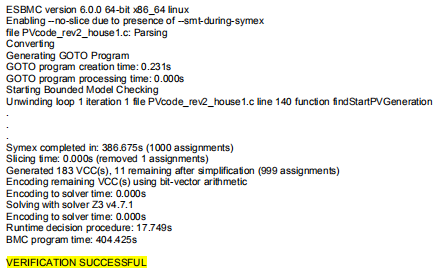
\includegraphics[width=0.65\textwidth]{esbmcverifh1.png}
\centering
\caption{Report generated by ESBMC (with Z3 solver) after validation of House 1.}
\label{fig:esbmcverifhouse1}
\end{figure}

However the $1,200$ W PV system (house $5$) failed (SAT) in line $337$ of the code, thereby indicating that the system is \textit{incorrectly} sized; in particular, the counterexample provided by the verification engine indicated that the nominal current from the charge controller is less than the minimum current demanded by the PV system, therefore the equipment chosen is not suitable to meet the design requirements.

Fig.~\ref{fig:esbmcverifhouse5} shows the report issued by the tool, with red highlights for the result, showing the incompatibility of the sized charge controller and the minimum necessary. The report generated by ESBMC was a text file of $14.1$ kB of size and $353$ lines of length. This verification took less than $1$ s to be performed, as indicated in the last line of Table~\ref{cases}, and it is faster than the previous analysis because ESBMC stops during the sizing check, which is in line $3$ of Algorithm~\ref{alg:verification-algorithm}, and does not perform the rest of verification code.

\begin{figure}[h]
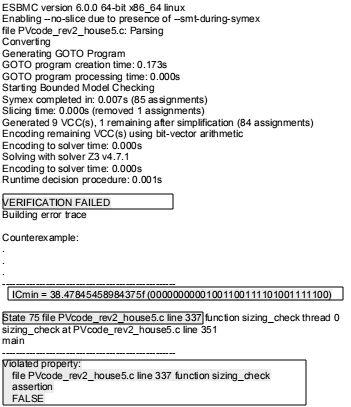
\includegraphics[width=0.5\textwidth]{esbmcverifh5.png}
\centering
\caption{Report generated by ESBMC (with Z3 solver) after validation of House 5.}
\label{fig:esbmcverifhouse5}
\end{figure}

%At the terminal, the command used to perform the verification is:
%\$ esbmc filename.c -\phantom{}-no-bounds-check -\phantom{}-no-pointer-check -\phantom{}-no-div-by-zero-check -\phantom{}-unwind 300 -\phantom{}-smt-during-symex -\phantom{}-smt-symex-guard --z3
%
%Where:
%
%\begin{itemize}
%\item The first three parameters, after the filename, are related to options that are usual to find bug in software, %for example, like bound check to arrays, pointer check, and division by zero, 
%but unnecessary to check at this kind of problem (if not removed, there is lost of performance during the automated verification);
%\item The parameter $unmind$ tells to ESBMC the limit to unroll the loops. This number was optimized (empirically) in order to reduce the running time and avoid to unwind unnecessarily the loops;
%\item The two parameters with $symex$ tell to ESBMC to perform an incremental SMT solving. There are other options, but this parameter is necessary because the complexity of the algorithms. The incremental SMT solving uses few RAM memory, compared with other SMT solving. 
%During empirical tests of the algorithms, the incremental solving was the only one who do not demanded 100\% the RAM memory. The use of swap-memory, i.e., the use of hard disk, reduces the performance and must be avoided;
%\item And the last parameter says to the tool that the Z3 SMT solver will be used.
%\end{itemize}
%

\subsection{CBMC}

Concerning the CBMC tool, similar results were obtained, but with some slower time than ESBMC. The experimentation returned SAT or UNSAT to all the case studies, i.e., it was conclusive to all houses. 

Related to the 700 W PV systems (house $1$, house $2$, house $3$, and house $4$), the tool could not reach an error in all the four houses and the execution time took from $18$ m $36$ s to $19$ m $02$ s. 

Fig. \ref{fig:cbmcverifhouse1} shows part of report produced by CBMC when validating the house 1. The file produced by CBMC is $270,512$ lines long and $39$ MB of size. The author highlighted the result, which shows that was not found design flaws within the bound $k$ of $100$.

\begin{figure}[h]
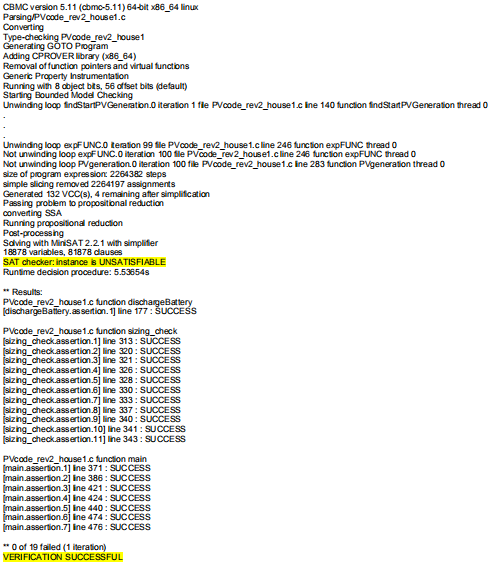
\includegraphics[width=0.8\textwidth]{cbmcverifh1.png}
\centering
\caption{Report generated by CBMC after validation of House 1.}
\label{fig:cbmcverifhouse1}
\end{figure}

However the $1,200$ W PV system (house $5$) failed (SAT) in line $337$ of the code; with the same counterexample presented by ESBMC. This verification took less than $1$ s to be performed as well. Fig.~\ref{fig:cbmcverifhouse5} shows the (edited) report produced, with the highlights about the flaw found: the minimum controller current needed to the PV systems is not compatible with the chosen controller of the sized system. The report file generated contains $217$ lines and it was $13$ kB of size.

\begin{figure}[h]
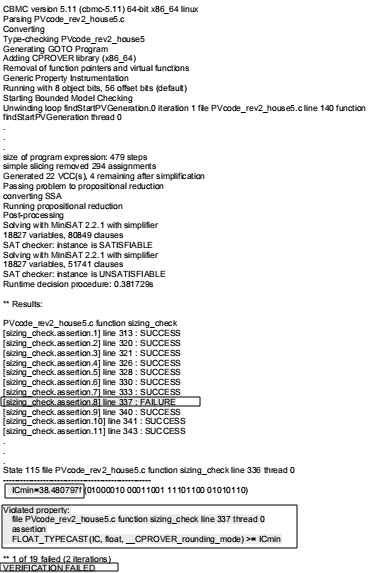
\includegraphics[width=0.7\textwidth]{cbmcverifh5.png}
\centering
\caption{Report generated by CBMC after validation of House 5.}
\label{fig:cbmcverifhouse5}
\end{figure}


\subsection{CPAchecker}

Finally, the CPAchecker tool presented some different results. Even using two different configuration possibilities, as described in Section~\ref{sec:setup}, the verification engine presented an UNKNOWN result for all the $700$ W systems (house $1$, house $2$, house $3$, and house $4$). 

This is because the \textit{time out} limit was reached, i.e., after $4$ hours of execution the tool was unable to decide if the verification was SAT or UNSAT. This is shown in Fig.~\ref{fig:cpavalidh1} is shown one of the text reports issued by CPAchecker. Differently of ESBMC and CBMC, CPAchecker produces a lot of different reports, notable for log, statistical, and counterexample files (which is graphical and not in text format).

\begin{figure}[h]
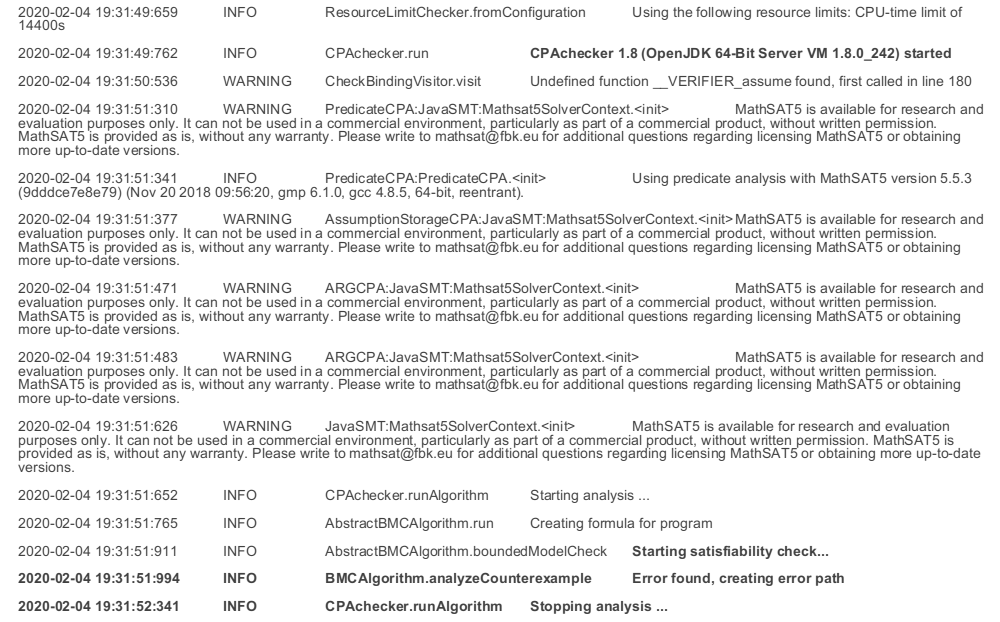
\includegraphics[width=0.8\textwidth]{CPA_verif_h1.png}
\centering
\caption{CPAchecker time out result for house 1 validation (file CPALog.txt).}
\label{fig:cpavalidh1}
\end{figure}

However, when validating the $1,200$ W PV system (house $5$), the tool presented a SAT message equal to the other engines, but with a execution time of $6$ seconds. Fig.~\ref{fig:cpavalidh5} show the result, with highlights to the line that causes the fail ($IC_{min}$) and part of the CFA (control-flow automata, represented as a control-flow graph) diagram pointing to this fail.

\begin{figure}[h]
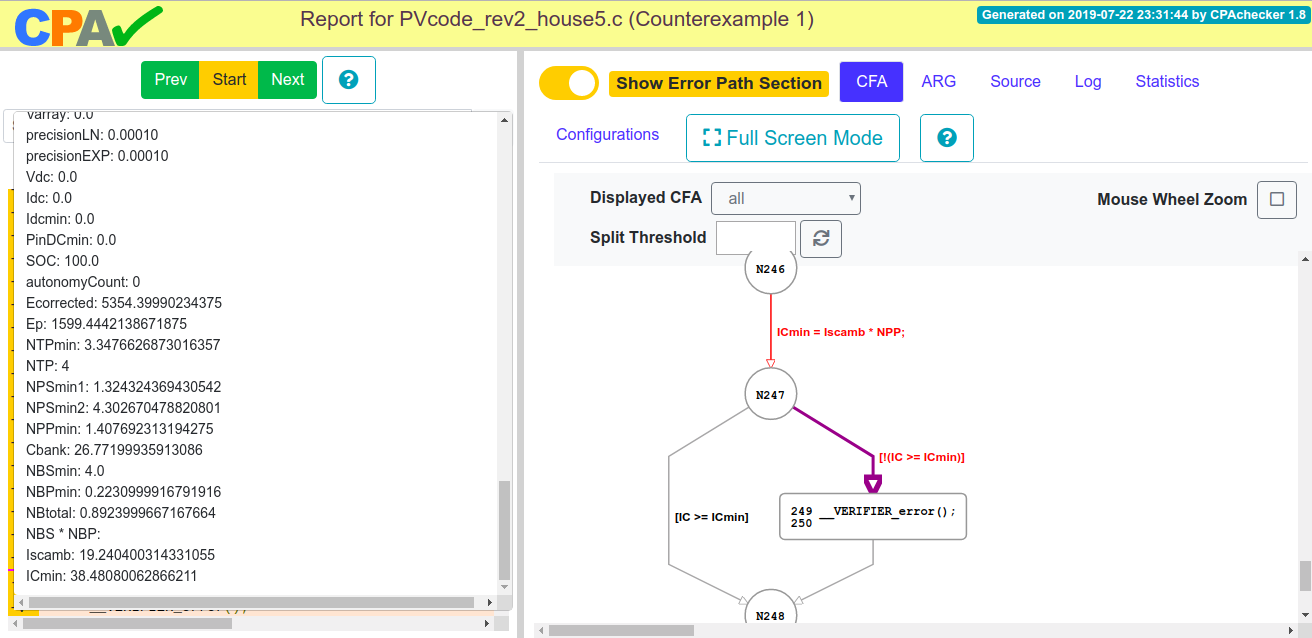
\includegraphics[width=1.0\textwidth]{CPA_verif_h5.png}
\centering
\caption{CPAchecker time out result for house 5 validation (file Counterexample.html).}
\label{fig:cpavalidh5}
\end{figure}


\subsection{HOMER Pro Specialized Simulation Tool}
\label{sec:homerenviron}

HOMER Pro is a powerful specialized electrical systems simulator, however even with the simulation characteristic, it in fact performs optimization when a given design is inputted to the schematic of the tool. This means that HOMER does not maintain the characteristic of the system under evaluation. It starts with the inputted information, however it uses the optimization default set up to increase or decrease the characteristic of each component until the load be meet by the electric generation system, and with the lowest cost. 

Therefore, in order to perform a limited simulation and not exceed the values of each component (for example, the total power of the PV array under evaluation), it is necessary use the 'search space' instead of 'HOMER Optimizer' for sizing. That is done at the menu of each component inputted in the schematic of the tool. 

Related to PV panels and batteries: If you want to simulate a particular capacity for PV and battery, you can use the 'search space' instead of 'HOMER Optimizer' for sizing. You can either aggregate all the PV panels together as a single PV component (in this case, the search space must vary from 0 to 1, i.e., from the option without PV panels until reach the power inputted to the component in the HOMER schematic) or add each PV components to represent the series configuration. For the batteries, you will have to find the equivalent capacity of the series and parallel configuration since HOMER considers only one battery component per simulation even if you add multiple battery components in the schematic.

Other drawback of HOMER Pro is the fact that the user cannot set the autonomy of the batteries as HOMER controller will decide when it is economical to discharge the batteries during the simulation year. Therefore, any simulation regarding battery autonomy is not possible to be evaluated.

Therefore, related to the comparative proposed, four $700$ W PV systems (houses $1$, $2$, $3$ and $4$) were evaluated by HOMER Pro (RQ2). The simulation results showed that for everyone of the sized systems, HOMER Pro concluded that it was not found feasible solution with the components inputted in the schematic. Fig. \ref{fig:homersimuh2no} shows one of the screens presented by HOMER Pro software, specifically to house $2$.

\begin{figure}[h]
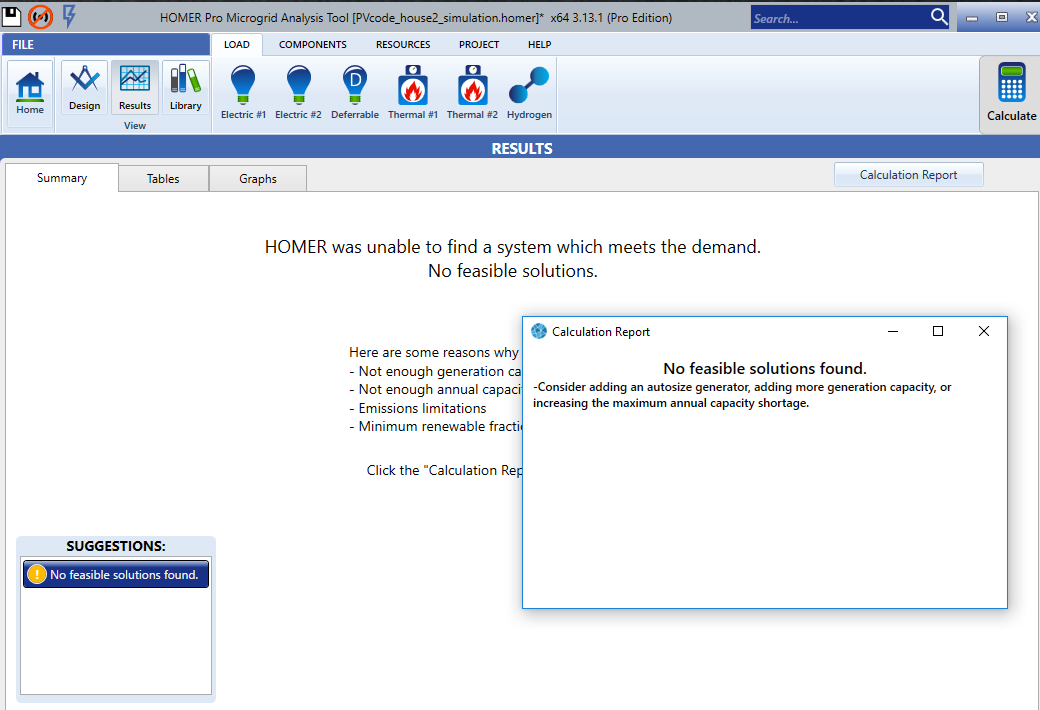
\includegraphics[width=0.8\textwidth]{homersimuh2no.png}
\centering
\caption{HOMER simulation screen presented for house 2 with no feasible solution found.}
\label{fig:homersimuh2no}
\end{figure}

Moreover, in order to evaluate what was the problem associated with the lack of feasible solution, it was performed some empirical changes to the evaluated project. Fig.~\ref{fig:homersimuh2yes} shows that a configuration with higher battery capacity (3 strings of 2 batteries each, 2S-3P, of 220 Ah; instead of 2 strings of 2 batteries each as the original sized system) can solve the problem of house 2. The same happened to the other tree houses of $700 W$, when improved battery capacity is presented by HOMER Pro as a optimal solution.

\begin{figure}[h]
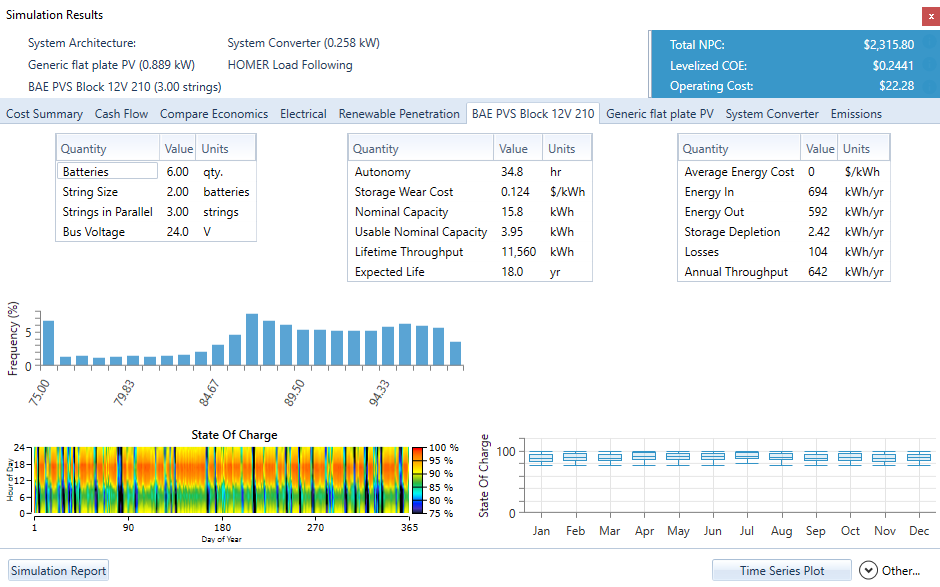
\includegraphics[width=0.8\textwidth]{homersimuh2yes.png}
\centering
\caption{HOMER simulation screen presented for house 2 with feasible solution.}
\label{fig:homersimuh2yes}
\end{figure}

The case study that was not possible to simulate was the $1,200$ W (house $5$). The reason is based on the fact that HOMER Pro do not allow to set up a battery autonomy (because it always size and optimize the electrical system in order to meet the load requirements for a entire year of simulation); therefore, it was was not possible to obtain any indication about the failures of this specifically PV system with simulation (RQ2).  

%
%Note that a PV design always uses daily average values of sun hours to each site, with impact in the PV components. Those hours are based on historical data and, in field, it is not unusual to find days where that number of hours was not reached due to weather conditions. The season has impact since the case studies are from the rain forest, where clouds are always present. As a result, the identified flaws in houses 1, 2, 3, and 4, are justified once again.
%
%We have evaluated five case studies in total using the HOMER Pro tool and our automated verification tool. Related to the HOMER Pro, the simulation, based on NASA data from the deployed systems (temperature and solar irradiance), shows that the restrictions were met by four 700 W PV systems (house 1, 2, 3 and 4), without any indication of sizing error or even performance. The case study that was unsuccessful during simulation was the 1,200 W (house 5); however, without any indication about the failures of this PV system. All the simulations took less than 5 seconds (each) to be performed.
%
%However, related to the results of the automated verification: (a) the 1,200 W PV system (house 5) failed during the sizing check. The number of panels was \textit{incorrect}; in particular, the counterexample provided by our verification method indicated 3 panels in parallel and the sized project has 2 in series and 2 in parallel. That verification took 63.3 hours to be performed. Surveying the owner of the 1,200 W system it was identified that, in fact, the system mostly of the time do not met the battery autonomy (mainly when all the loads are turned on). That behavior is expected because the system was purchased as an off-the-shelf solution and not as a specific design for the electrical charges of the house; (b) Related to the four 700 W PV systems, just one verification finished its analysis (house 1) considering the time-out of 432 h of computing. The sizing check was successful during automated verification, but there was found flaw related with the battery autonomy, when SOC reached levels below of 75\%. The automated verification identified the flaw right after the first night-discharge cycle, before the solar system start to recharge the batteries. The proposed tool took 409.3 hours to find this error at house 1. This possible flaw was confirmed with the dweller that uses the system: at least once or twice a mouth is usual the system to turn off, normally during raining days or with more clouds in the sky, and after the sun rises the system returns to normal operation. Related to houses 2, 3 and 4, it was considered that the automated verification had a time-out condition, with no conclusive results.

\subsection{Comparing Automated Verification and Simulation Results with Real PV Systems}

There were divergence of results for the houses $1$, $2$, $3$ and $4$ w.r.t. of proposed approach: the automated evaluation shows that there is not project flaws, but simulation demanded to improve batteries capacity (adding one more string of batteries to the system). 

In order to evaluate which validation is correct, it was necessary to access the access interviews performed with the dwellers of deployed systems. From July of $2018$ to March $2019$, a monthly visiting was performed to apply surveys to the dwellers and to collect data from a local monitoring system: not every month were reported some energy interruption of the PV systems. 

However, even when one interruption is reported in a month, this represents around $3.33$\% of interruption for the entire period ($1/30$), which indicates $96.97$\% of availability of the PV system ($96.67\% = 100\%-3.33\%$) and it is in accordance to what was described in Section~\ref{sec:availability}, because the type of electrical load of the houses is not critical; this situation is considered an energy interruption, but is not considered a system flaw, further affirming RQ1. Therefore, the proposed approach using automated verification provides the correct evaluation of the PV system, thus answering RQ2.

House $5$ presented flaws from all tools (automated verified or simulation); however, only automated verification approaches indicated which design error was responsible for the flaw (charge controller specification), further answering RQ2.

In order to validate the possible flaw identified by the automated verification from house $5$, it was surveyed the owner of the $1,200$ W system. It was identified that, in fact, the system does not meet the battery autonomy when all loads are turned on, and this was double checked with the monitoring system from the charge controller, which showed that the maximum power or surge power were not exceeded, thus affirming RQ1; this behavior is expected since the system was purchased as an off-the-shelf solution and not as a customized design for the electrical charges of the house. 

%\begin{figure}[h]
%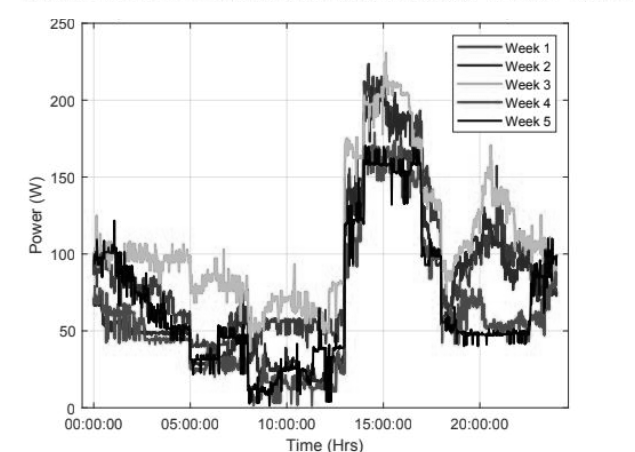
\includegraphics[width=0.65\textwidth]{loadcurve.png}
%\centering
%\caption{Five weeks monitored load curve from House 1.}
%\label{fig:loadcurve}
%\end{figure}
%
%\subsection{Experimental results}
%\label{sec:results}
%---------------------------------------------------
\section{Threats to Validity}
%---------------------------------------------------

At this Chapter, it was reported a favorable assessment of the proposed method. % over a diverse set of real-world benchmarks. 
Nevertheless, it was also identified five threats to the validity of the results that can further be assessed.

\textit{Model precision:} each component of the PV system is mathematically modeled. %, and the precision of the proposed method depends on the precision of that particular model. 
The adoption of more complex models, or even an evaluation in a PV laboratory to validate the model could add more reliability to the results.

\textit{Time step:} The run-time complexity of the proposed method is an issue; the time step of one hour can be further reduced to approximate the algorithm to the real-world scenario.

\textit{Case studies:} The case studies are performed only in one municipality. A more complete evaluation can be performed with more case studies.

\textit{Simulation Tool:} Only HOMER Pro was used. The inclusion of other specialized simulation tool or even a general simulation tool that uses the same mathematical model adopted by the automated verification could change the comparative.

\textit{Temperature and Solar Irradiance Data}: Information related to temperature and solar irradiance of each case study, independently of using simulation or formal verification, come from databases available online~\cite{Temperature, Irradiance}. However, considering that riverside communities do not have weather stations, the data used in the present study come from the closest municipality (Manaus in all case studies), where stations collect regularly those data. Therefore, the most accurate should be the use of weather stations in each location.

\section{Conclusion}

This Chapter showed in details how the state-of-art computer science method of automated verification was adapted in order to be used in stand-alone solar PV systems to validate their behavior. Moreover, is was possible to picture the comparative of how the proposed method and the traditional one of simulation work differently.

Detailed diagrams, flowcharts and algorithms with pseudo-code were presented with the aim to support the proposed work and to facilitate the understanding. And even more so, the assumptions adopted for the automated verification and simulation software were listed.

Furthermore, at this Chapter it was performed the comparative among verifiers with the proposed automated verification using model checking, which showed that 'incremental' ESBMC had the best overall performance. CBMC presented the same results, however with a worse time to result, and CPAchecker was not conclusive (house $1$, house $2$, house $3$, and house $4$) because the \textit{time out} was not enough to obtain some result.

A comparative with a specialized simulation tool was performed as well, however some limitations of the tool, mainly related to not allow battery autonomy setup or the oversize of the batteries bank by HOMER Pro, restricted the comparative between automated verification tools versus simulation tools.

Based on the fact that all case studies were deployed at the field, with regular visiting to perform interview with the dwellers, and with monitoring system in some of the houses (house $1$, house $2$, house $3$, and house $4$), it was possible to compare the computational validation (by simulation or automated verification) with the real world employment of the stand-alone solar PV systems. The final conclusion was that the proposed tool is sound and with an acceptable performance. 
